
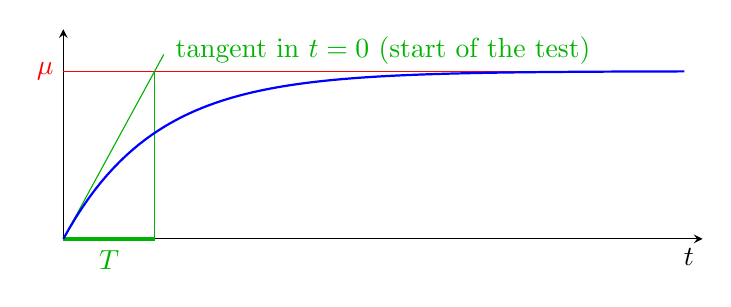
\begin{tikzpicture}
\pgfplotsset{width=0.8\columnwidth,height=0.35\columnwidth}



\begin{axis}[
       ymin=0,
       ymax=1.25,
       xmax=7,
       xlabel={$t$},
       every axis x label/.style=
         {at={(current axis.right of origin)},
          anchor=north,xshift=-5},
       axis x line = bottom,axis y line = left,
       ticks=none,
       clip=false,
]

\draw[red]
     (axis cs:0,1) --
     node[pos=0,left]{$\mu$}
     (axis cs:6.8,1);
\draw[green!70!black]
     (axis cs:0,0) --
     node[pos=1.02,right]{tangent in $t=0$ (start of the test)}
     (axis cs:1.1,1.1);
\draw[green!70!black]
     (axis cs:1,1) --
     (axis cs:1,0);
\draw[green!70!black,ultra thick]
     (axis cs:0,0) --
     node[pos=0.5,below]{$T$}
     (axis cs:1,0);

\addplot [blue,thick,domain=0:6.8, samples=100]
         {1-exp(-x)};
\end{axis}


\end{tikzpicture}
